\chapter{Propuesta de Solución}
La solución propuesta es crear una herramienta que permita a los turistas de cierta zona turística de México poder localizar zonas o áreas de interés, así como realizar recorridos turísticos; utilizando el GPS de su dispositivo móvil y trazando áreas de interés (geovallas) dentro de dichas zonas turísticas. En el presente capítulo se describirán los componentes que forman parte de la solución propuesta. 

\section{Arquitectura de Solución}
Se desarrollará una aplicación la cual contará con módulos móvil y módulos web que, la cual tendrá una arquitectura como se muestra en la Figura \ref{fig:arquitecturaPropuesta}, dicha aplicación ayudará al sector turístico ya que proporcionará información sobre rutas turísticas y áreas de interés de una localidad en particular.

\begin{figure}[htbp]
	\begin{center}
		\hypertarget{fig:arquitecturaPropuesta}{
			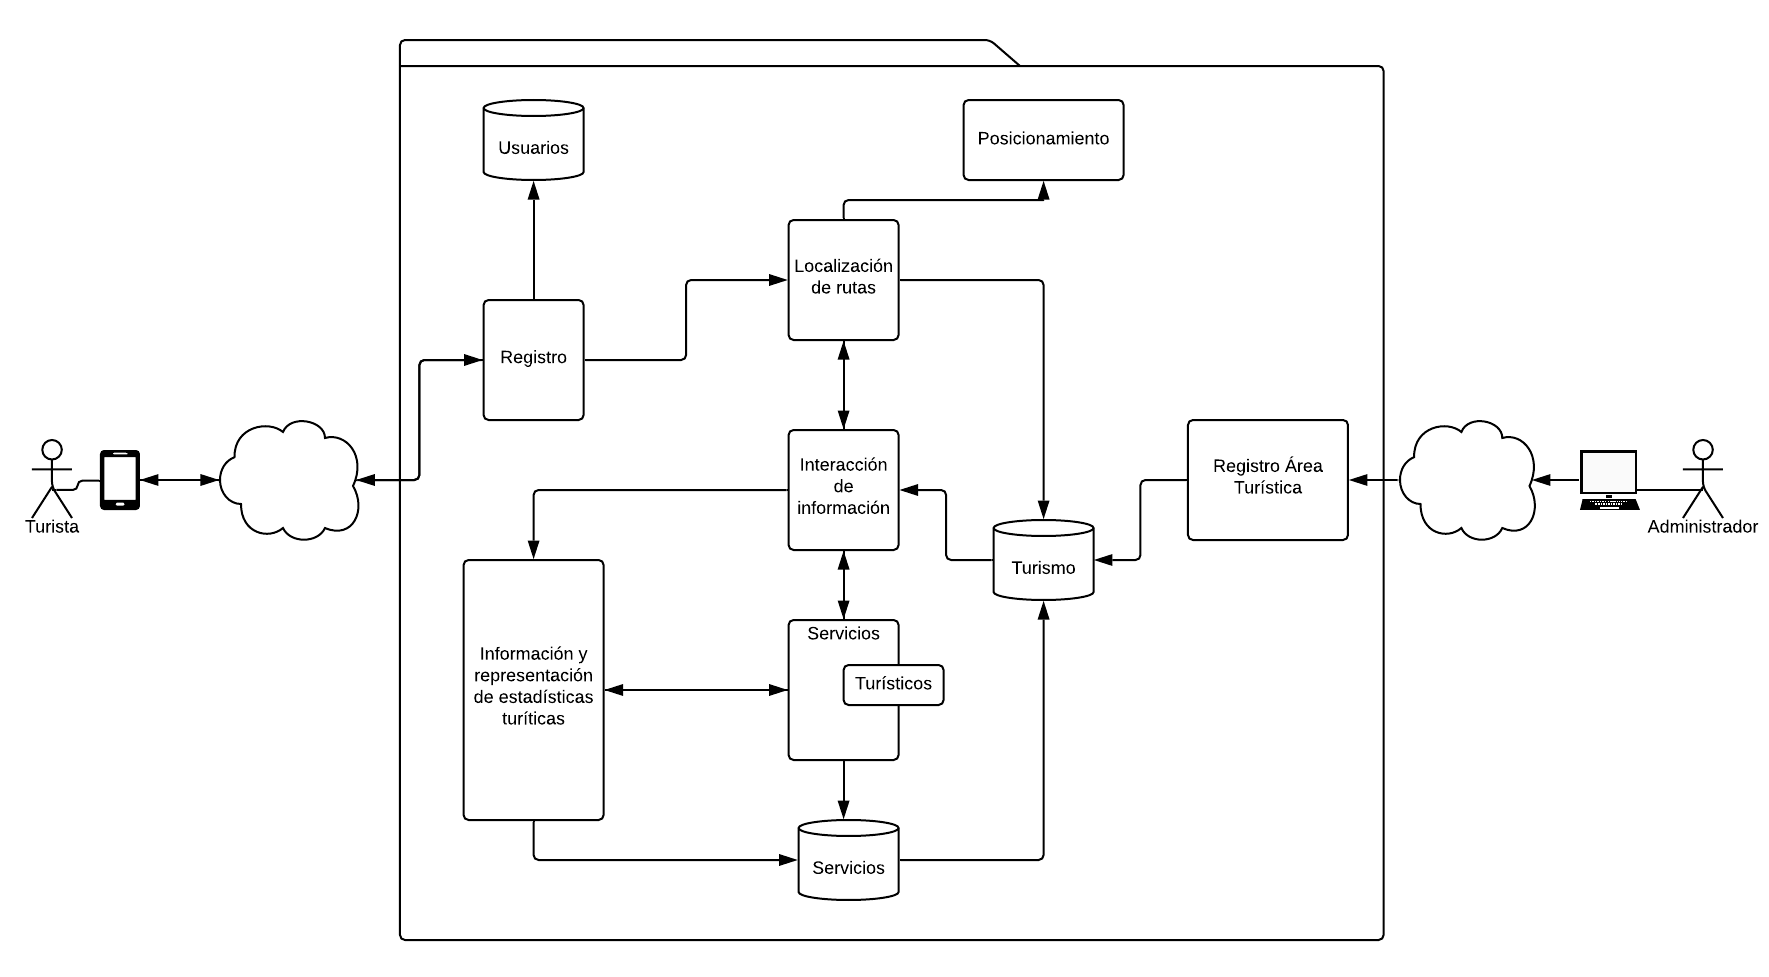
\includegraphics[angle=90, scale=.7]{propuestaSolicion/turismo/images/arquitecturaPropuesta}
			\caption{Arquitectura de propuesta de solución}
		}
		\label{fig:arquitecturaPropuesta}
	\end{center}
\end{figure}

\newpage
Como puede observarse en la Figura \ref{fig:arquitecturaPropuesta}: \hyperlink{fig:arquitecturaPropuesta}{Arquitectura de propuesta de solución}, la aplicación móvil propuesta para el Trabajo Terminal contará con dos actores: Turista y Administrador.\\

El actor \textbf{Administrador} será el encargado de hacer el registro de las áreas turísticas, esto a través de una aplicación web,  para que posteriormente el actor \textbf{Turista} pueda acceder a esta información mediante la aplicación móvil. \\

El actor \textbf{Turista} tendrá la posibilidad de registrarse en la aplicación para poder contar con el servicio que ésta ofrece, dentro de la aplicación se generarán rutas turísticas basadas en la localización del usuario y de esta forma podrá consultarse los servicios turísticos que se ofrecen dentro del área localizada.\\

Así mismo se contará con un módulo de \textbf{Información y representación de estadísticas turísticas} en el cual se trabajará con la información del usuario para la generación de rutas, sugerencia de sitios y servicios disponibles en la zona localizada.

\section{Módulos}

En esta sección se describirán los módulos que se contemplan para el desarrollo del sistema, el diseño de los módulos fue hecho con base en el análisis de requerimientos (más adelante en el capítulo \hyperlink{cv:analisisSolucion}{Análisis de la Solución} se detallará este proceso) y tomando en cuenta las necesidades que debe cubrir. Así mismo este diseño fue tomado en cuenta para la planeación de los Sprints a desarrollar durante todo el Trabajo Terminal. \\

A continuación se listarán los módulos contemplados para el sistema y una breve descripción de estos:

\begin{description}
	\item[Registro] Este módulo será mediante el cual los nuevos clientes de la aplicación se registrarán en ella para poder hacer uso de esta. 
	
	\item[Localización de rutas] Este módulo será el encargado de generar las rutas turísticas para los clientes de la aplicación, para ello depende del trazado de área de interés y del posicionamiento del cliente.
	
	\item [Posicionamiento] Este módulo se encargará de proporcionar la información de la posición en la que se encuentra el cliente, al módulo de \textbf{Localización de rutas}, cabe mencionar que para poder proporcionar el posicionamiento del cliente, este deberá encontrarse dentro del área de interés previamente trazada.
	
	\item [Interacción de la información] Dentro de este módulo se tratará la información proporcionada por el módulo \textbf{Localización de rutas}, \textbf{Registro de área turística} y \textbf{Servicios}, esta información servirá para trazar nuevas rutas turísticas en el módulo \textbf{Localización de rutas}, para identificar nuevos servicios turísticos o remover los que ya no se utilicen en el módulo \textbf{Servicios}, y por último proporcionará toda la información recabada al módulo \textbf{Información y representación de estadísticas turísticas}.
	
	\item [Servicios] Este módulo se encargará de identificar los servicios turísticos de la información proporcionada por el módulo \textbf{Interacción de la información}, y de igual manera se encargará de proporcionar información sobre estos servicios a los módulos: \textbf{Interacción de la información} e \textbf{Información y representación de estadísticas turísticas}.
	
	\item [Información y representación de estadísticas turísticas] En este módulo se recopilará la información de los módulos: \textbf{Interacción de la información} y \textbf{Servicios}; y se generarán estadísticas con base en esta información para proporcionarla de nuevo a los módulos anteriormente mencionados, y de esta manera generar las rutas turísticas.
	
	\item [Registro área turística] Este módulo será dirigido únicamente al administrador del sistema, ya que él será el encargado de hacer el registro de las áreas turísticas. Dentro de este módulo se registrará la información pertinente para poder realizar el trazado de rutas turísticas, así mismo será el módulo en el que se tracen las áreas de interés o geocercas.
\end{description}

Cabe mencionar que únicamente los módulos \textbf{Registro}, \textbf{Servicios}, \textbf{Información y representación de estadísticas turísticas} y \textbf{Registro área turística}, tendrán acceso a la base de datos del sistema. \\

Una vez que se definieron los módulos que contemplará el sistema se decidió utilizar la metodología SCRUM para el desarrollo del sistema. Dicho proceso será descrito en la siguiente sección.

\section{Módulos}

\section{Análisis de Viabilidad}

\subsection{Económico}

En México, la actividad económica se encarga de aportar casi el doble del promedio que contribuyen las economías de la Organización para la Cooperación y Desarrollo Económico (OCDE por sus siglas en español, u Organisation for Economic Cooperation and Development, OECD por sus siglas en inglés\footnote{De aquí en adelante se empleará OCDE para referirise a la Organización para la Cooperación y Desarrollo Económico}). Así mismo aporta el 8.7 \% del PIB del país\cite{ocde}. \\

Por otro lado, la industria turística ha crecido a nivel global, incluso por arriba de la economía mundial, sin embargo para asegurar la competitividad, sostenibilidad e inclusividad, se requieren políticas\cite{turismoEnMexico}.\\ 

El turismo en México es una actividad económica que tiene una gran importancia porque, como ya se mencionó, aporta un porcentaje alto en el PIB del país. Dado esto, México recibe anualmente un amplio caudal de turistas que provienen de todo el mundo y que genera un alto número de empleos locales\cite{importanciaTurismo}. \\

Según el análisis en el entorno económico y la relevancia del turismo en México, se puede llegar a la conclusión de que el país actualmente esta atravesando un excelente momento para el turismo, lo que demuestra la solidez y las excelentes expectativas que se tienen sobre la economía mexicana en el sector turístico.\\

\subsection{Técnico}

Para el desarrollo del proyecto se ha decidido hacer uso del trazado de áreas de interés (geovallas o geocercas), esta es una delimitación geográfica virtual que se hace a través de un programa de rastreo. El uso de esta tecnología permite administrar zonas o lugares que se encuentran dentro del área trazada o delimitada\cite{geovalla}. \\

Para la implementación del la geocerca existen algunas API's(Application Programming Interface, API por sus siglas en inglés\footnote{De aquí en adelante se empleará API para referirse a Interfaz de Programación de Aplicaciones}), las cuales pueden ser utilizadas para el desarrollo del proyecto, algunas de estas API's son: Navixy\footnote{\url{https://www.navixy.com/es/documentacion/guias-de-usuario/interfaz-web/monitoreo/herramientas-del-mapa/geocercas/}} y RedGPS\footnote{\url{https://www.redgps.com/blog-noticias/bienvenidas-las-geocercas-a-redgps-1}}. Por lo que la implementación de estas geocercas se puede realizar.

 \subsection{Legal}

De manera legal el proyecto es viable, ya que el usuario final es el que limita el uso de la geolocalización, es decir, no hay una ley en México que restrinja su uso\cite{geolocalizacion}. 


\section{Características}